\chapter{Introduction}
\label{cap:introduction}

\section{The evolution of HPC systems}
\textbf{High Performance Computing (HPC)} term refers to computer technologies
used in advanced software applications requiring large computing power. The
applications are usually parallel in order to run on large clusters of
machines, called \textbf{supercomputers}.

HPC systems are currently considered one
of the most important resources both in research and in industry; the raising
of performance-hungry scientific applications lead European Union and other
subjects to allocate huge amount of funds to HPC development. HPC is 
considered strategic
for Europe's future and essential for industry to innovate in products and
services \cite{EUstrategy}. However, the research is called to solve several
technological limits to the performance scaling, along with addressing
the problem of providing guarantees in terms system reliability too, as
described in the subsequent paragraphs.

The increasing number of computing nodes, thus CPU cores, the end of
Dennard's scaling \cite{esmaeilzadeh2011dark} and the moving towards Exascale
computing\footnote{see next section for the Exascale definition.} indeed
introduce numerous challenges, in particular regarding thermal and energy
optimizations, dependability and resilience concerns, resource allocation
scheduling, and parallel programming models \cite{shalf2010exascale}.

Currently, the main component of HPC infrastructure variable costs is related
to thermal and energy considerations. More power consumption means more
electricity costs and heat dissipation, more heat dissipation means higher
cooling needs and consequently again more electricity costs. Considering the
large numbers of servers in HPC clusters, introducing an optimization in a
small part of the system may lead to not negligible economical
and environmental advantages. In fact, Exascale requires strong efforts in all
related fields, from the infrastructure to the software in the direction of
increasing power efficiency and programmability.

\begin{figure}[t]
		\centerline 
{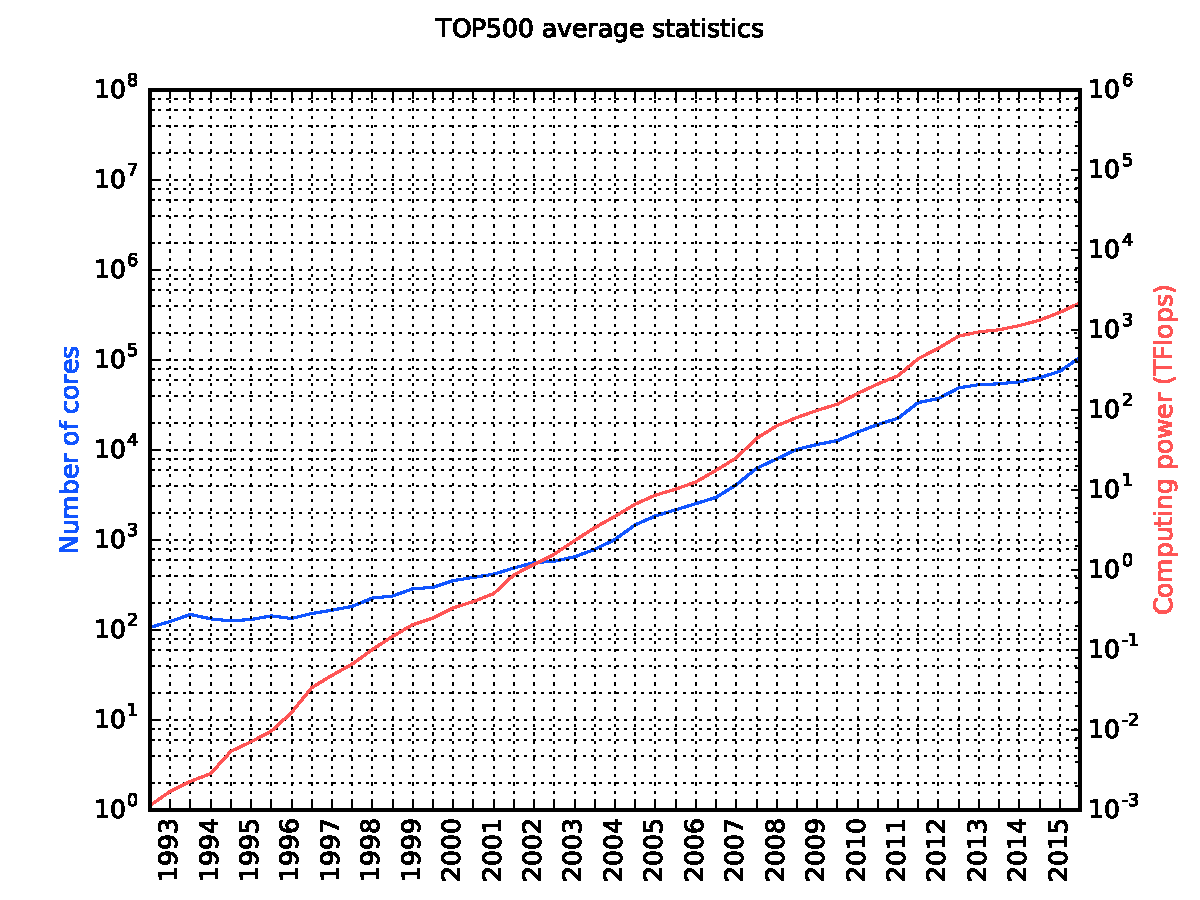
\includegraphics[scale=0.7]{img/cap1-top500-avg-comp}}
		\caption[TOP-500 supercomputers average performance]{Average number of cores and computing power of TOP-500
		supercomputers (TOP500.org data, retrieved 5 August 2016)}
		\label{fig:corestrend}
\end{figure}

\begin{figure}[t]
		\centerline 
{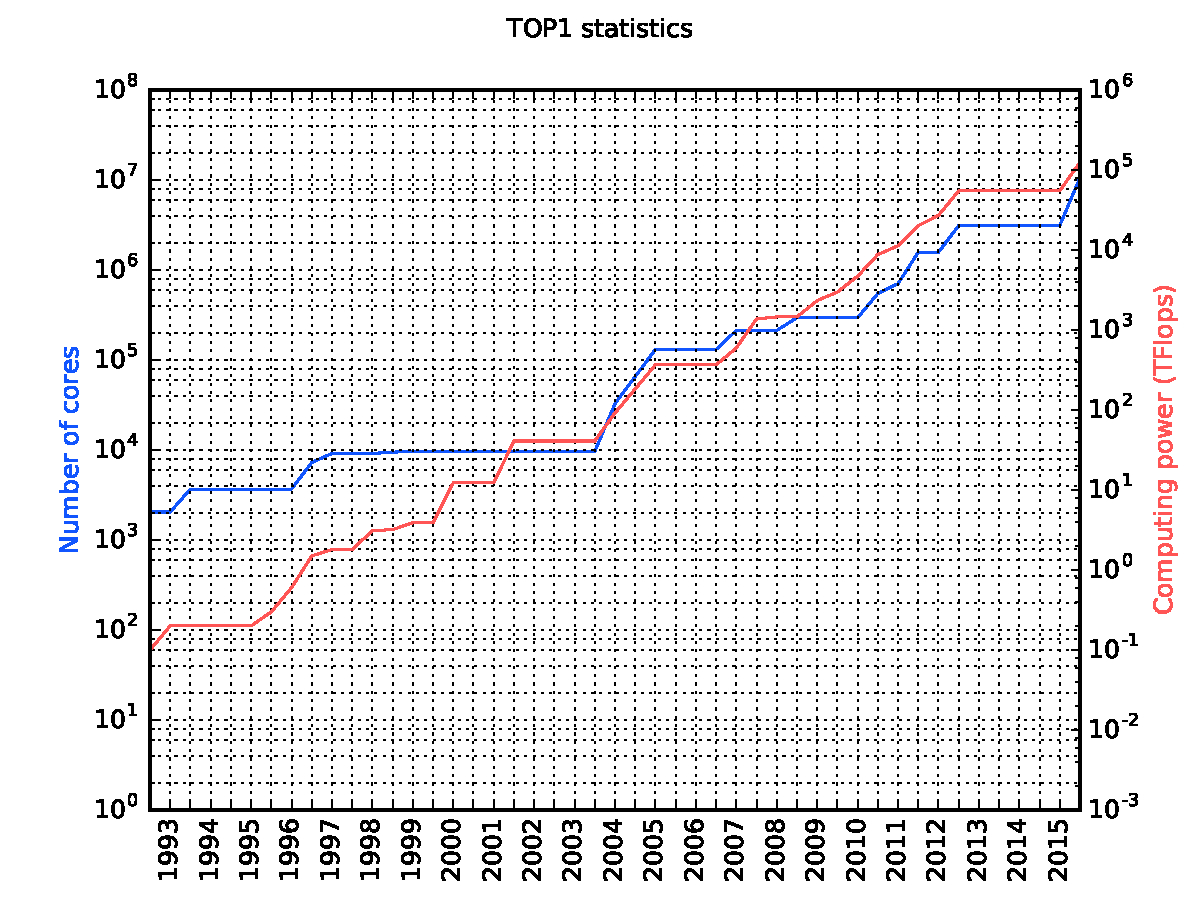
\includegraphics[scale=0.7]{img/cap1-top500-max-comp}}
		\caption[TOP-1 supercomputers performance]{Number of cores and computing power of the TOP-1
		supercomputer (TOP500.org data, retrieved 5 August 2016)}
		\label{fig:corestrend2}
\end{figure}


In last decades the rapid development of processing units maintained
acceptable levels of power consumption while increasing the performance
delivered. The computational units and computational power trends over
past two decades is shown in Figure \ref{fig:corestrend} and Figure
\ref{fig:corestrend2}.

Unfortunately, the miniaturization of semiconductors cannot go on forever,
thus the End of the \emph{Moore's Law} is one of the big concern. In fact,
the plateauing of voltage levels and the increasing of leaking current is
leading to a power wall \cite{Villa2014}.
The reduction of the performance increasing
trend, or even the reaching of a performance plateau, would significantly slow
down the scientific research \cite{snir2011exascale}. In 2014, the Department
of Energy of United States planned to achieve the too ambitious goal of
Exascale with 20 MW of power in 2018 \cite{USExascale}, but later the deadline
was extended.

\subsection{Exascale as a key goal to reach}
\textbf{Exascale computing} refers to systems having a minimum computing power
of more than 1 exaFLOPS, i.e. \( 10^{18} \) FLOPS.

Research towards Exascale is not limited to the computer science domain, but it
strongly affects all the areas of science and engineering. The increasing
complexity of mathematical models and the growing size of Big Data requires
a growing amount of computing resources.

The Exascale goal is in fact of great interest for a wide range of
applications. We can mention several examples, like the study of astrophysical phenomena, weather forecasting, product market simulations, the development of
new drugs, the analysis of health risks, etc.
\cite{Reed:2015:ECB:2797100.2699414}. For all these applications, Exascale
would enable the possibility of deploying more complex mathematical models,
capable of providing much more accurate and reliable results.


%%%%%%%%%%%%%%%%%%%%%%%%%%%%%%%%%%%%%%%%%%%%%%%%%%%%%%%%%%%%%%%%%%%%%%%%%%%%%%%
Vice versa, other non-computer scientists
are studying to find alternative technologies to the current one, in order to
mitigate the today issues. Several physicist are studying new types of
semiconductors, for instance the very promising research on silicon photonics
\cite{6476868}.

From the previous considerations we can state that HPC is still a very hot
topic of research and solving the related problematics is not just a matter
of computer science, but it will influence and it will be influenced by
the research activities in almost all fields.

%%%%%%%%%%%%%%%%%%%%%%%%%%%%%%%%%%%%%%%%%%%%%%%%%%%%%%%%%%%%%%%%%%%%%%%%%%%%%%%


\subsection{HPC systems architecture}
Since HPC systems require by definition high computational capabilities, the
computational resources are typically distributed across different high-end
machines (nodes). They are connected via a high speed networks, typically
10Gigabit Fiber Optics Ethernet or InfiniBand.

The storage is also provided through distribution solutions like
Storage Area Network (SAN) or Network Attached Storage (NAS).
Both solutions have to be designed for
HPC environment. In particular, the storage performance and capacity
should possibly scale linearly with the numbers of nodes and disks.

\begin{figure}[t]
		\centerline 
{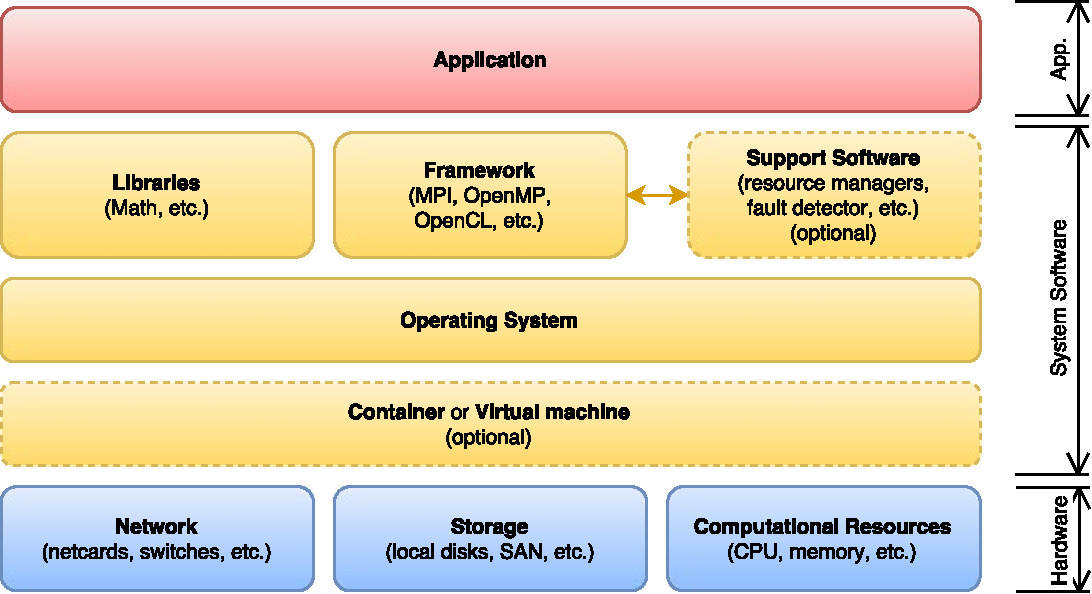
\includegraphics[scale=0.7]{img/cap1-generalarchitecture.pdf}}
		\caption[General architecture of a HPC node]{The general architecture of one node in a HPC system.}
		\label{fig:generalarchitecture}
\end{figure}

The general architecture of a single node in a HPC cluster is shown in
Figure \ref{fig:generalarchitecture}. End-user applications run over
a stack of software and, in particular, exploit the API provided
by a specific parallel programming framework like MPI or OpenMP. Since the
application computational requirements are far behind the performance
capabilities provided by a single CPU, the application must be designed in
order to run multiple threads or processes. Parallel frameworks
simplify the development of the applications, providing suitable API to
manage the execution of multiple tasks, the communication and the
synchronization among them.

Furthermore, the application may use other library providing specific
functionalities (e.g. math functions) or interact with
other software frameworks, like resource managers. The operating system as
usual provides to all of software the abstraction of the hardware (virtualized
or not).


\section{Dependability issues in HPC}
In HPC, dependability - a broad term including reliability, resilience,
fault tolerance, etc. - is another possible future wall in reaching
Exascale computing \cite{5871590}. To highlight the
size of the problem is sufficient to say that the Mean Time To Failure (MTTF)
for current HPC systems is way below 100 hours \cite{egwutuoha2013survey}.

The research community is therefore focusing its effort towards five key
directions \cite{cappello2014toward}:
\begin{enumerate}
\item statistical and technical characterization of hardware faults;
\item development of a standard fault interface from hardware to software;
\item improving fault prediction, containment, detection, notification and recovery;
\item the development of programming abstractions for resilience, especially fault-tolerant algorithms;
\item proposing fault-tolerant approaches both in hardware and software design.
\end{enumerate}

In this work, we focus on the item 4 proposing a tool that can be used
in HPC parallel applications in conjunction with a fault-detection mechanism to
support fault-tolerant executions on distributed systems.


\subsection{Fault-Tolerance requirements and techniques}
As already presented, one of the most important discussed theme in HPC is the
dependability concern. In particular, since the MTBF is very low compared
to the applications timespan, it is required fault-tolerance techniques
able to guarantee the termination of the application even if one or more faults
occur. In fact, some HPC applications take days or weeks to terminate and
after a fault a restart from the beginning is not acceptable. Therefore,
fault-tolerance is no longer a \emph{nice-to-have} feature, but it became a
\emph{mandatory} one in HPC systems.

To highlight the previous considerations, a simplification of
the Mean Time To Failure (MTTF) and Mean Time Between Failure calculus (MTBF)
is proposed, with the objective to provide a trivial qualitative analysis.
Assuming the system non repairable, thus \( \text{MTTF}=\text{MTBF} \),
let's consider a cluster of 1.000 CPUs Intel Xeon processor of E7 Family that has \(\text{MTTF}=100.000h\) (\textasciitilde 11y) \cite{E7Reliability}. The overall MTTF can be calculated as:

	\begin{equation}\label{eq:mttf1}
		\lambda_i = \frac{1}{\text{MTTF}_i}
	\end{equation}
	\begin{equation}\label{eq:mttf2}
		\lambda_{\text{overall}} = \sum{\lambda_i}^n
	\end{equation}
	\begin{equation}\label{eq:mttf3}
		\text{MTTF}_{\text{overall}} = \frac{1}{\lambda_{\text{overall}}}
	\end{equation}

Applying (\ref{eq:mttf1}), (\ref{eq:mttf2}), (\ref{eq:mttf3}) to our scenario:
\[  \text{MTTF}_{\text{overall}} = \frac{1}{ 1.000 \cdot \frac{1}{100.000} }
 = 100h \]

The overall MTTF was drastically reduced from 11 years to just few days.
Please also note that modern supercomputers have more than 30.000 physical
CPUs, leading to MTTF to be less than 4 hours. It is clear that most of the
HPC applications, that requires more than few hours to conclude, need a
sort of abstract of a fault-free system, in order to execute ideally without
being affected by hardware faults. Several approaches have been proposed in
literature and industry. The state of the art of this techniques will be
discussed in the next chapter.

\subsection{Failures taxonomy and sources}
Following the classification provided by \emph{Snir et al.}
\cite{snir2014addressing}, the HPC failures may be grouped in three
categories: \emph{detected and corrected by the hardware} (DCE), \emph{detected
but not corrected by the hardware} (DUE) and \emph{non-detected silent errors}
(SE).
We do not consider DCE, since they are transparent to the software; for
instance, the ECC memory correction is an example of DCE and it is usually
performed transparently to the software. We neither deal with SE: the
correctness of the result has to be checked by the application since the
framework has no tool to infer it.

In the example about the calculation of MTTF, the CPU fault rate was
considered. However, other components like memory may be the source of
the failure, further deteriorating the reliability. Regarding \textbf{hardware faults}, they can be divided -
following the \emph{Snir et al.} classification - in \emph{compute soft},
\emph{compute hard}, \emph{network}, and \emph{I/O} errors. Vice versa,
\textbf{software faults} can be classified in: \emph{pure software}, 
\emph{hardware propagating up}, and \emph{software propagating down} errors. 
This taxonomy is better presented in the subsequent 
Table \ref{tab:faulttaxonomy}.


\begin{table}[ht!b]
\centering
\begin{tabular}{ c|c|c}

\multirow{4}{*}{\parbox{2.5cm}{\vspace{2cm}Hardware faults}} 
 & \centering Compute soft errors & \parbox{6cm}{\vspace{.5\baselineskip}
 Errors caused by transient
 faults in electronics,  e.g. memory corruptions caused by an electromagnetic
 interference
 \vspace{.5\baselineskip}}
 \\ \cline{2-3}
 & \centering Compute hard errors & \parbox{6cm}{\vspace{.5\baselineskip}
 Permanent fault of a
 computational component (CPU, RAM, etc.) due to a physical problem, e.g.
 electromigration.
 \vspace{.5\baselineskip}}
 \\ \cline{2-3}
 & \centering Network errors & \parbox{6cm}{\vspace{.5\baselineskip}
 Total or partial loss of network
 connectivity, often caused by external component w.r.t. machine, e.g.
 network apparatus failures.
 \vspace{.5\baselineskip}}
 \\ \cline{2-3}
 & \centering I/O errors & \parbox{6cm}{\vspace{.5\baselineskip} Transient or
 systematic errors during
 the reading or writing to disks or other storage
 \vspace{.5\baselineskip}} \\ \hline
\multirow{3}{*}{\parbox{2.5cm}{\vspace{1.3cm}Software faults}} 
 & \centering Pure software errors & \parbox{6cm}{\vspace{.5\baselineskip}
 The category containing the
 classical programming issues: correctness errors, concurrency errors, etc.
 \vspace{.5\baselineskip}}
 \\ \cline{2-3}
 & \centering HW propagating to SW & \parbox{6cm}{\vspace{.5\baselineskip}
 A bug in the hardware that
 propagates up to the software, typical an unmanaged DUE.
 \vspace{.5\baselineskip}}\\ \cline{2-3}
 & \centering SW propagating to HW & \parbox{6cm}{\vspace{.5\baselineskip}
 A bug in the software that
 damages the hardware; it is typical of firmware in embedded appliances.
 \vspace{.5\baselineskip}}\\ 

\end{tabular}

\caption[The fault taxonomy in a HPC environments]{The fault taxonomy in a HPC system according to
\emph{Snir et al.} classification.}
\label{tab:faulttaxonomy}

\end{table}


The number of possible faults that may lead to a failure in the system
and/or in the running HPC applications explains why the thematic of fault
tolerance is today not only bound to the embedded world, but it has a
fundamental importance also for HPC environments.

\subsection{Checkpoint/Restart}
In response to these faults, most of long-run jobs require a
\textbf{Checkpoint/Restart (C/R)} mechanism. The C/R paradigm
consists in performing periodic \emph{checkpoints}, i.e. save the
status of the system on non-volatile memory, in order to \emph{restart} the job if a fault occurs. The restart
is triggered after the fault is detected and corrected.

Provided the images are saved in a persistent storage
\footnote{In this context \emph{persistent storage} is intended as fault-free
non-volatile memory.}, this
technique guarantees the ability to recover from any type of fault.
However, the cost of checkpoint is extremely high and it has to be executed
periodically. The overhead can easily reach 50\% of the total execution time,
reducing considerably the impact on the efficiency of the system
\cite{fiala2012detection}.

\subsection{Performance variation and degradation}
Performance variation and degradation are increasing problems in
semiconductors. The component aging has an important effect in
these two problematics.

In HPC, not only faults have to be taken in account: the performance
degradation and fluctuation affect also the overall performance of the
jobs. Then, it makes important to preserve an acceptable level of aging
of all components, through periodical maintenances. Unfortunately,
most of operations on machines require to shutdown it; in this direction,
migration allows a system administrator to request the freeing of a machine
without  the necessity to wait the completion of current tasks or freeze
entirely the job via C/R.

\section{Resource management in HPC}
The resources management in supercomputers is a prominent challenge. 
Resource allocation in HPC is a problem studied since 1980s, trying to
find a model to allocate jobs in optimal distribution across supercomputers.
Albeit the question is old, the increasing of resources spread over several
nodes and the diversity of the
software require specific policies to schedule and allocate jobs over the
cluster. In this regard, we may choose between applying static or dynamic
policies. Static policies are in most cases suboptimal or totally inadequate
to manage parallel workloads. While dynamic policies allows us to adapt
resource allocation decisions to the current workloads characteristics and
system status. Moreover, heterogeneous computing
is considered by AMD one of the essential capabilities to reach
Exascale computing \cite{7155462}.

The goal of this policies may be vary, for instance obtain the maximum
performance for certain category of applications or reduce the
resource underutilization to minimum, in order to maintain an efficient system.
Different applications may have different priorities or they have to generate
results (e.g. predictions) within a given mandatory rate. In this case, it's
more important to satisfy the strongest
requirement than to have the maximum efficiency.

Most of the large clusters are utilized not only for HPC, but also for Cloud
Computing. This mixed environment requires to manage different types of
workloads: resource-intensive long-run for HPC applications and a resource
flexible adjustment for Cloud. Resource management techniques capable of
dealing with mixed workload are consequently required \cite{chen2013dynamic} for large computing centers.

In 2016 \emph{Cela et al.} provide an overview \cite{cela2016fostering} of
energy-related issues in new exascale HPC applications. Resource management
at MPI level is considered essential in order to achieve high scalability.
One of the main topics proposed for future research is precisely the migration
of MPI processes, that is the main topic of this work. Migration opens up a 
wide range of possibilities. For instance the resource manager can adapt the
computing resource assignment to time varying application performance
requirements. Moreover, the application load can be balanced among the system
nodes, in order to level down the power consumption and the temperature peaks.

This thesis presents a novel migration technique in MPI and its integration and
exploitation in Barbeque RunTime Resource Manager, a resource manager part of the BOSP open source project.

\section{Message Passing Interface}
The \textbf{Message-Passing Interface} standard (abbreviated in MPI) is
the \emph{de-facto} standard for parallel computing across different
nodes. 
The MPI Forum - composed by both academic and industrial
people - released the first version of this standard in 1994 and the last
version (3.1) was released in 2015\cite{mpistd}. 

The MPI standard describes the syntax and the semantics of function calls in
the Application Program Interface (API) provided by a MPI library to the user
software. This API allows the communication, the management and the
coordination between processes of a parallel application. MPI is mainly
used for distributed computing, despite in theory it can be used for the
execution on local machine only. In the latter case, \emph{OpenMP} is usually
preferred, since it is optimized specifically for single node executions.
To reach better performance, most applications are implemented combining
the usage of MPI and OpenMP together.

The MPI standard is written through
a language-independent specification, in order to be implemented in any
programming languages. The most common languages are C, C++ and Fortran.

\begin{figure}[t]
		\centerline 
{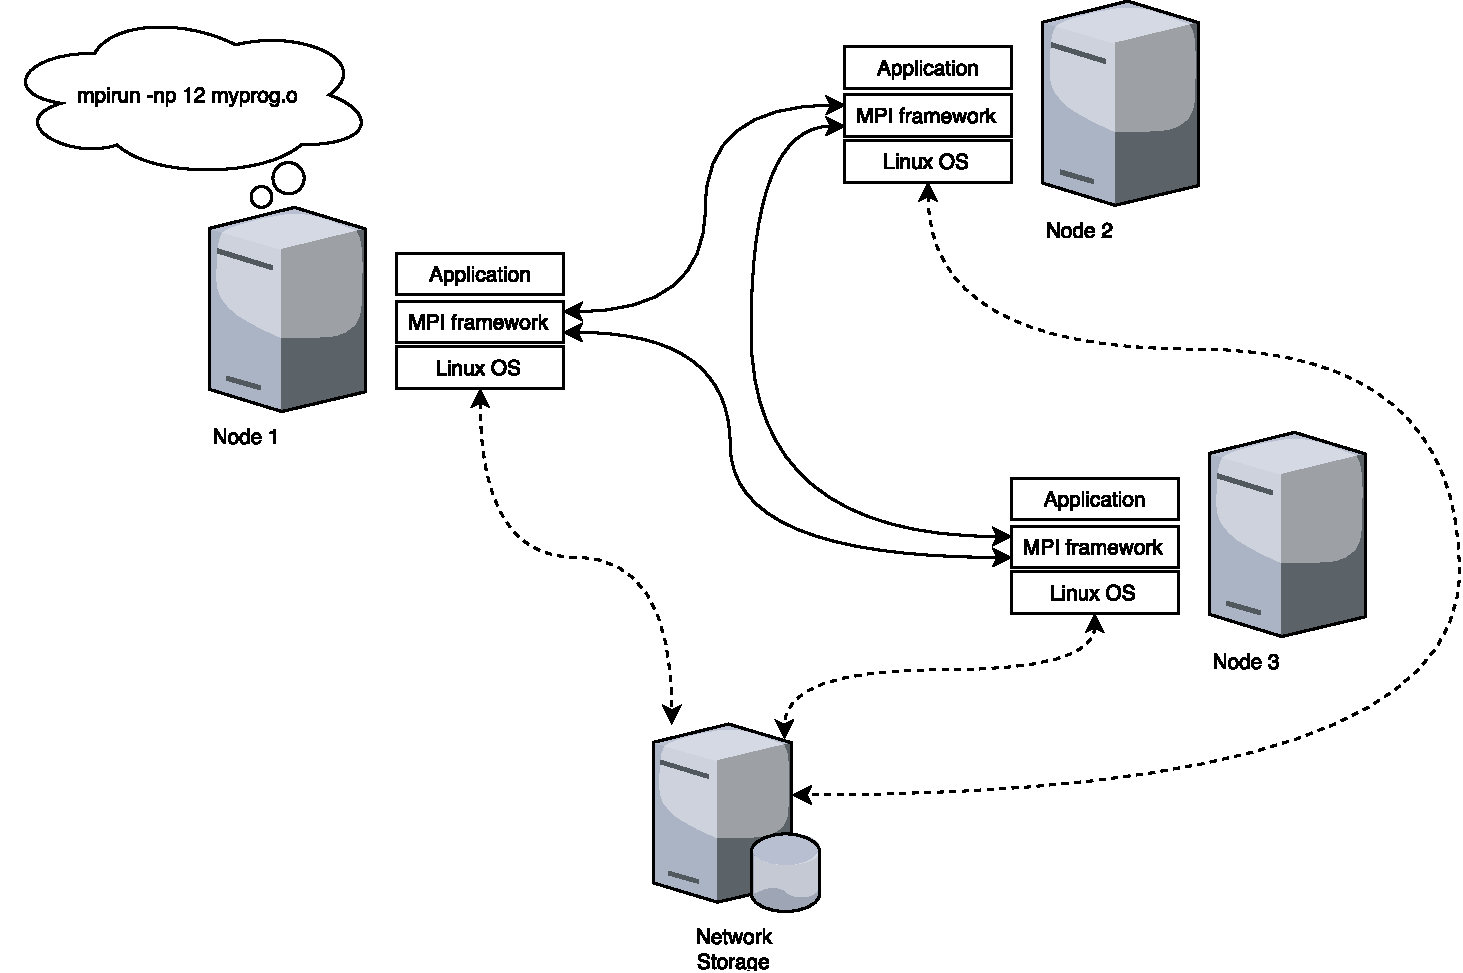
\includegraphics[scale=0.5]{img/cap1-mpiarchitecture.pdf}}
		\caption[MPI systems typical setup] {A typical configuration of MPI systems: the user launches the
		\texttt{mpirun} command on Node 1 that distributes the computation
		also over the Node 2 and Node 3. All nodes have access to a common 
		network storage to get the program and the data.}
		\label{fig:cap1-mpiarchitecture}
\end{figure}


\subsection{MPI Application Execution Flow}
A MPI typical MPI execution is presented in Figure 
\ref{fig:cap1-mpiarchitecture}. The user launches the job via the
\texttt{mpirun} command, then the MPI framework spawns the processes
in the other available machines (how this is performed is implementation
dependent).

The application must be linked with the static or dynamic library of MPI,
that provides \texttt{MPI\_*} function calls. Usually every program starts
with \texttt{MPI\_Init} and ends with \texttt{MPI\_Finalize}. Both functions
are implementation-dependent, but in general \emph{MPI\_Init} performs some
setup required before any other MPI routines and the
\texttt{MPI\_Finalize} coordinates the execution conclusion freeing the
allocated resources.

The communication between processes is divided in two categories:
\emph{point-to-point} (direct communication between two processes) and
\emph{collective}
(communication one-to-many or many-to-many). The latter is performed through
the coordination of the various MPI frameworks on all nodes. A typical example
of collective feature is the \emph{barrier}: every program should synchronize
at the same point before continuing.

Having a common set of functions allows to perform easily and equivalently
benchmarks of the same application on different MPI frameworks or to port
the program on another framework without refactoring the code.

\subsection{MPI implementations}

Today, several implementations of MPI are available, among which we cite
the two most commonly used: MPICH\cite{karonis2003mpich} and Open
MPI\cite{gabriel2004open}. They are both open source and have reached a good
level of stability even with a considerable number of features, thanks to the
very active communities and the large funding of big companies and
universities.

The history of MPICH can be split in two part: MPICH-1 and MPICH-2. The
development of the latter (at a later time called simply MPICH) starts in
2001 to add the feature of MPI version 2 and subsequently version 3 to MPICH-1.

Open MPI represents the union of three
previous implementations: LA-MPI, FT-MPI and LAM/MPI. The third 
was extensively used in research literature. All of which ceased their
development shortly after the begin of Open MPI project in 2003.

The two implementation mainly differs in the purpose of application: MPICH is
a very stable basis and standard reference for the development of special
purpose needs. Open MPI targets more general cases and it already offers
several pre-implemented features, e.g. different types of network
communication channels and topology.

Since our framework is supposed to be a general tool that tries to address
the issues of the most of HPC applications, we selected the Open MPI
implementation to develop the feature presented in next sections. Furthermore,
the extreme high modularity of Open MPI internal code was a big advantage in
the development of \texttt{mig} framework\footnote{Note that the keyword
`framework` may generate misunderstanding: as explained in Chapter
\ref{cap:design}, the \texttt{mig} framework is a module of Open MPI, not a new
MPI framework}.


\section{Migration of MPI processes}
This thesis presents a technique implemented in Open MPI able to allow the
migration of MPI processes among different nodes of the cluster. Moving a
process across different machines is not a straightforward task and
it constitutes a specific research topic. This work exploits existing
process migration tools applying them to Open MPI for HPC applications.

Migration of processes can be exploited to solve or mitigate some of the
previous presented issues. Obviously, the migration is not for free and
introduces an overhead that must
be taken in account, while being triggered by an appropriate software, for
instance by a fault detector or a resource manager.

Migration is particularly interesting for resource management: current runtime
resource managers in HPC are limited to assign resources during the application
startup, therefore they are not usually able to reschedule the application over
different nodes. Migration adds the capability of rescheduling to resource
managers, that they have to take in account the significant overhead of
moving processes between two nodes.

In large clusters the topology and consequently the location of the processes
of the same job significantly impacts on overall performance; even if
all nodes are in the same network, the distant of two machines noticeable
affects the network performance. If the topology of the cluster changes -
despite the application is not involved - a rescheduling may be convenient
to reach better performance. Since C/R is too expensive in terms of time and
required resources, this scenario can be an interesting exploitation of
migration techniques.

Regarding fault tolerance, the migration may in fact lead to a the reduction
of the number of C/R required:
an appropriate pre-fault detection system would trigger the migration if an
imminent fault is detected, avoiding the long restart required if the fault
happens.

Certainly, a sudden unexpected undetectable fault is not manageable with
a migration technique. This is why C/R mechanisms cannot be fully replaced.
Instead, the frequency of the checkpoints can be effectively reduced,
provided an appropriate fault probability analysis.

The software architecture considered for this work does not provide a fault
detector, but assume the presence of an external one that signals the resource
manager in case of imminent fault. Subsequently, the resource manager and the
MPI framework will trigger the migration. With this setup, the resource
manager is the only interlocutor with the MPI framework and it can allocate
and possibly reallocate resources over available nodes.

\section{Thesis structure and objectives}
The main topic of this thesis is a novel approach to process migration
implemented in Open MPI. This technique was also presented at the EuroMPI 2016
conference\cite{myEuroMPI}. In addition, the exploitation of this technique
with the \textbf{Barbeque Run-Time Resource Manager} (from now simply
\emph{BarbequeRTRM}) is presented in conjunction with a basic centralized
resource management policy for distributed systems.

In Chapter \ref{cap:state-of-the-art} the State of the art related to
migration and C/R techniques is discussed and the novelty of the
proposed method is highlighted. The Open MPI and CRIU frameworks are
described in Chapter \ref{cap:ompicriu}. Subsequently in Chapter
\ref{cap:design} and \ref{cap:integration} the design, the implementation and the integration with
\emph{BarbequeRTRM} are explained, detailing and arguing all design choices.
The testing results are discussed in Chapter \ref{cap:evaluation}, focusing on
the introduced overheads. Eventually, in Chapter \ref{cap:discussion} future
research directions and developments are proposed. It is also the thesis end containing the conclusions.   
